\begin{figure}[!t]
\begin{center}

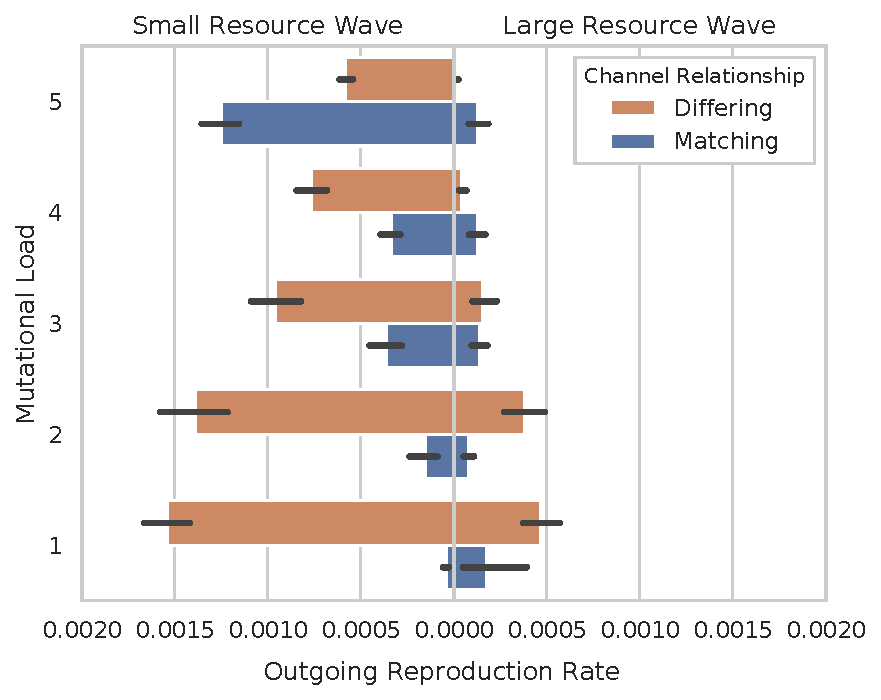
\includegraphics[width=\columnwidth]{title=reproductive_labor+_data_hathash_hash=4a000b28acccbd08+_script_fullcat_hash=970b6aa9f7815573+_source_hash=d53f428-clean+ext=}

\caption{
Reproductive cooperation phenotypes by treatment between updates 5000 and 50020.
Small resource wave treatments are plotted on the left half of the plot, facing leftwards.
Large resource wave treatments are plotted on the right half of the plot, facing rightwards.
Mutational load increases in the upwards direction.
Bar height represents the mean per-update rate at which cells reproduce and replace a neighbor with their daughter cell, killing that neighbor.
Each two-tone pair of bars compares this rate with respect to neighbor cells that have matching channel ID and neighbor cell that do not.
Orange bars represent the rate at which cells reproduce over different-channel neighbors and blue bars represent the rate at which cells reproduce over same-channel neighbors.
Error bars represent 95\% confidence intervals.
The net outgoing reproduction rate (e.g., the sum height of bar pairs) differs by treatment because the net resource harvest rate, and therefore net cellular reproduction rate, depends on channel group configuration.
} \label{fig:reproductive_labor}
\end{center}
\end{figure}
